\chapter{Theory, Design and Simulation}
\label{sec:chapter_2}

The fundamental concepts of an OFDM design is described. A detailed block diagram is shown. A theoretical basic based band OFDM system is compared with IEEE 802.11 standard scheme. Influential parameters to are explained with guided us to have other parameters in Table \ref{table:sys_param}. Arrangement of the IEEE 802.11a carriers demonstrated.\\
A short discussion of Carrier Frequency Offset is initiated and its origin and the impacts on the whole system on receiver side and a possible solution to reduce the issue is discussed.\\

\section{OFDM System Architecture}
Generally, an OFDM signal is defines as a summation of many OFDM standard symbols, which can considered continuous in the time domain.It can be defined as following:\\

\begin{equation} \label{general_form}
\begin{split}
s(t) =\sum\limits_{k=-\infty}^{+\infty} s_{k}(t)
\end{split}
\end{equation}

where $s_{k}(t)$ is the k-th OFDM symbol which starts at time $t= t_{s}$. An OFDM system is a multi-carrier transmission mechanism which the mathematical model is generalized by the summing a series of modulated subcarriers digitally. This modulation can be phase shift keying (PSK) or quadrature amplitude modulation (QAM) and transmitted in parallel. So, we can  conclude:\\
\begin{equation} \label{ofdm_digital_mod}
\begin{split}
s_{k}(t)=
\left\{
	\begin{array}{ll}
	Re\left( \sum\limits_{i=-\frac{N}{2}}^{\frac{N}{2}-1} d_{i+\frac{N}{2}} \exp\lbrack j2\pi(f_{c} - \frac{i+0.5}{T})(t- t_{s})\rbrack\right) , & t_{s}\le t < t_{s} + T\\
	0, & \mbox{otherwise}
	\end{array}
\right.
\end{split}
\end{equation}

where $T$ is the symbol duration, $N$ is the number of subcarriers, $f_{c}$ is the signal carrier
frequency on the radio frequency (RF) band, and $d_{i}$ is the complex value for PSK or QAM modulated symbol. We reach $I_{i}$ and $Q_{i}$ being the in-phase and quadrature part of $d_{i}$, respectively.\\
The complex envelope of an OFDM signal given by the following equation is used as the baseband notation:
\begin{equation} \label{ofdm_complex_env}
\begin{split}
s_{k}(t)=
\left\{
	\begin{array}{ll}
	Re\left( \sum\limits_{i=-\frac{N}{2}}^{\frac{N}{2}-1} d_{i+\frac{N}{2}} \exp\lbrack j2\pi\frac{i}{T}(t- t_{s})\rbrack\right) , & t_{s}\le t < t_{s} + T\\
	0, & \mbox{otherwise}
	\end{array}
\right.
\end{split}
\end{equation}

The real and imaginary parts of \ref{ofdm_complex_env} are the in-phase ($I$) and quadrature ($Q$) of the baseband OFDM signal. Consequently, they are multiplied by a cosine and a sine waveform with a carrier frequency to generate the passband OFDM. At the receiver, each subcarrier is down-converted with a subcarrier of the desired frequency and supported over the symbol period. For example, the complex value for the $m$-th subcarrier $d_{m}$ is obtained equation \ref{m_th_carrier}, where the whole signal is multiplied by the frequency of $\frac{m}{T}$, and then integrated over the symbol period $T$:
\begin{equation} \label{m_th_carrier}
\begin{split}
\int\limits_{t_{s}}^{t_{s} + T} s_{k}(t) \exp \lbrack -j2\pi \frac{m}{T} (t-ts) \rbrack dt & = \int\limits_{t_{s}}^{t_{s} + T}  \left( \sum\limits_{i=-\frac{N}{2}}^{\frac{N}{2}-1} d_{i+\frac{N}{2}} \exp\lbrack j2\pi\frac{i}{T}(t- t_{s})\rbrack\right) \exp \lbrack -j2\pi \frac{m}{T} (t-ts) \rbrack dt\\
& = \sum\limits_{i=-\frac{N}{2}}^{\frac{N}{2}-1} d_{i+\frac{N}{2}} \int\limits_{t_{s}}^{t_{s} + T}  \left( \exp\lbrack j2\pi\frac{i-m}{T}(t- t_{s})\rbrack\right) dt\\
& = Td_{m+ \frac{N}{2}}
\end{split}
\end{equation}

\ref{m_th_carrier} shows all the subcarriers over the integral region are zero except the desired one. The desired output for the signal demodulation, $d_{m+ \frac{N}{2}}$ multiplied to a constant factor $T$, is exactly the integration for the $m$-th subcarrier. Since each subcarrier has an exact integer number of cycles within OFDM symbol duration, the orthogonality between subcarriers is guaranteed.\\
the mathematical model for discrete time signal is as below if the OFDM symbol is sampled with a sampling period $\dfrac{T}{N}$:
\begin{equation} \label{math_model}
\begin{split}
s(n)= s_{k}(\frac{nT}{N})= \sum\limits_{i=0}^{N-1} d_{i} \exp(j2\pi\frac{in}{N}), n= 0, 1, ... , N-1
\end{split}
\end{equation}

This represents an inverse DFT (IDFT) for PSK or QAM symbols.  See Figure \ref{fig:io_idft}.\\

\begin{figure}[h!]
\centering
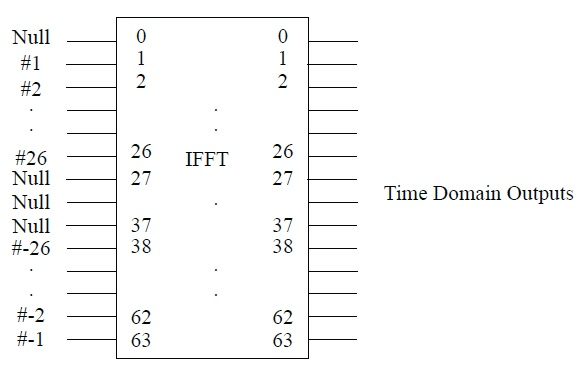
\includegraphics[width=10cm]{content/fig/io_idft.JPG}
\caption{Input and Output of IDFT \cite{802_11}}
\label{fig:io_idft}
\end{figure}

Figure \ref{fig:ofdmsystemmodel} presents the OFDM system block diagram. The first block represents the data source. They are the bits which an application may send. In the simulation it is realized by a random and fixed bit generator. The following QPSK modulation block converts this bits into symbols, which are complex numbers. Each symbol carries several bits. The third block is the first one actually relevant for OFDM. The serial symbol stream is converted into a channel and OFDM symbol structure. In the simulation it is represented in a matrix shape where the rows are different channels and each column is an OFDM symbol. This means that each OFDM symbol, formed by $c$ (\#channels) serial symbols (complex numbers), is distributed over the $c$ channels.\\

\begin{figure}[tbp]
\centering
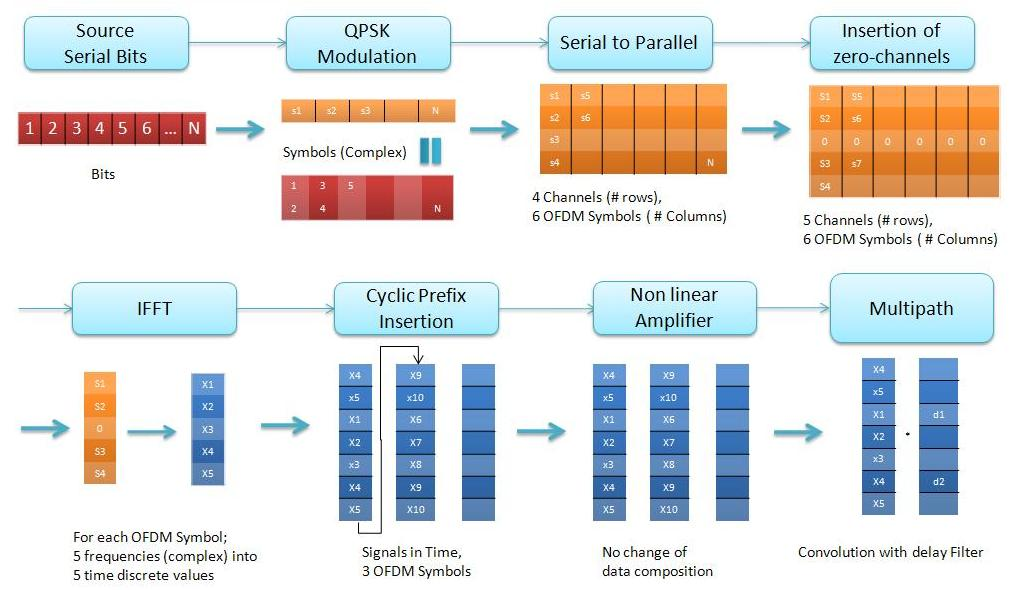
\includegraphics[width=\textwidth]{content/fig/ofdmmodel1.JPG}
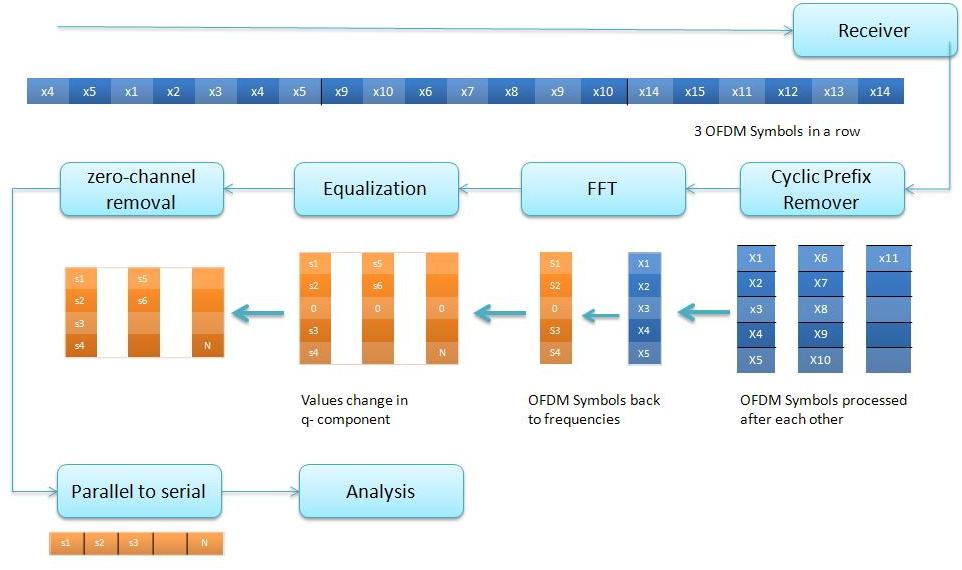
\includegraphics[width=\textwidth]{content/fig/ofdmmodel2.JPG}
\caption{OFDM System Model}
\label{fig:ofdmsystemmodel}
\end{figure}

In the next step zero channels are added in order to separate well subsequent OFDM symbols. For the simulation structure zero rows are added in the middle of the matrix. The following block interprets each symbol (complex number) of an OFDM symbol as a orthogonal frequency and converts each OFDM symbol per IFFT into a vector of time discrete values of the same length. As sixth step the cyclic prefix insertion is done. In order to maintain orthogonality of the frequencies but prevent ISI, an amount of \textit{guard values} are copied from the end of each OFDM symbol to its beginning. The number of rows in the simulation matrix grows by that by the number of \textit{guard values}.\\

The following block is the NLA which depends on the optimization parameter $\beta$ (back-off). At this point the transmitter side ends. In order to simulate the multipath a convolution is made on each OFDM symbol with the delay filter. Since the simulation is made on each OFDM symbol separated, this operation works with a memory in order simulate a serial transmission.\\
The receiver side is just the opposite of the transmitter. In the cyclic prefix remover the copied values are deleted and the simulation matrix size decreases. The next block performs the FFT on each OFDM symbol which reconstructs the as frequencies interpreted complex numbers.\\ The following equalization block tries to remove the effect of the multipath. For the simulation a multiplication with the inverted transfer function of the multipath is operated. By this, only the phase of the complex symbols changes.\\ 
Finally, the zero channels are removed and the matrix structure is reconverted to a series of symbols. The following analysis is done on the received symbols and consequently they are not demodulated into a bit-stream.\\
According to the above analysis, the basic architecture for a baseband OFDM system that contains the essential parts is shown in Figure \ref{fig:basic_ofdm}.\\

\begin{figure}[h!]
\centering
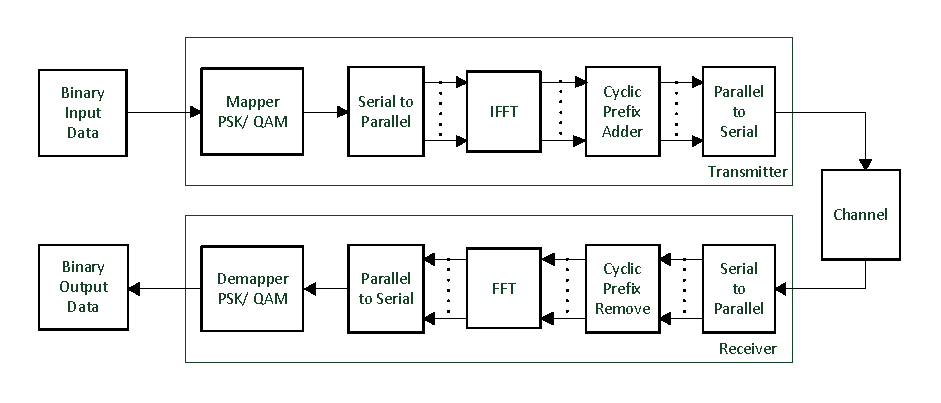
\includegraphics[width=\textwidth]{content/fig/basic_bb_ofdm.pdf}
\caption{Basic baseband OFDM system}
\label{fig:basic_ofdm}
\end{figure}

In practice, to prevent sharp transactions at the sample time boundaries, a windowing block is used for filter shaping. In conclusion, spectrum utilization is enhanced dramatically. Therefore, the baseband OFDM symbol can be written as below:\\
\begin{equation} \label{ofdm_window}
\begin{split}
s_{k}(t)=
\left\{
	\begin{array}{ll}
	w(t - t_{s})\sum\limits_{i=-\frac{N}{2}}^{\frac{N}{2}-1} d_{i+\frac{N}{2}} \exp\lbrack j2\pi\frac{i}{T}(t- t_{s}- T{g}) , & t_{s}\le t < t_{s} + (1+\beta)T_{sym}\\
	0, & \mbox{otherwise}
	\end{array}
\right.
\end{split}
\end{equation}

where $T_{g}$ is the guard interval duration, $T_{sym}= T+ T_{g}$ is the OFDM symbol period,
symbol starting time $t_{s}= kT_{sym}$, and $w(t-t_{s})$ is the pulse shaping window, which is
usually a raised cosine filter, and $\beta$ is the roll-off factor.\\
The OFDM mechanism is used in 802.11 and Wimax standards. \cite{802_11} It has good tolerance against multipath and the receiver is easier to implement. We will see the details of implementations in practical systems.\\


\section{OFDM Specifications in IEEE 802.11a Standard}

\subsection{Introduction of IEEE 802.11}
The Institute of Electronic and Electrical Engineers (IEEE) has released IEEE 802.11 in June 1997. The standard defined physical and MAC layers of wireless local area networks (WLANs).\\
The physical layer of the original 802.11 standardized three wireless data exchange techniques:

\begin{itemize}
  \item Infrared (IR);
  \item Frequency hopping spread spectrum (FHSS);
  \item Direct sequence spread spectrum (DSSS).
\end{itemize}


The 802.11 radio WLANs operate in the $2.4 GHz$ ($2.4$ to $2.483 GHz$) unlicensed Radio Frequency (RF) band. The maximum isotropic transmission power in this band allowed by FCC in US is $1 Wt$, but 802.11 devices are usually limited to the $100 mWt$ value.

The physical layer in 802.11 is split into Physical Layer Convergence Protocol (PLCP) and the Physical Medium Dependent (PMD) sub layers. The PLCP prepares/parses data units transmitted/received using various 802.11 media access techniques. The PMD performs the data transmission/reception and modulation/demodulation directly accessing air under the guidance of the PLCP. The 802.11 MAC layer to the great extend is affected by the nature of the media. For example, it implements a relatively complex for the second layer fragmentation of PDUs.\\


\begin{figure}[h!]
\centering
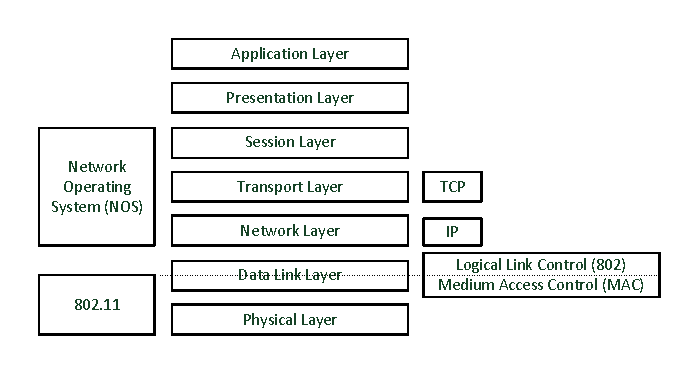
\includegraphics[width=\textwidth]{content/fig/osi_ref_mdl.pdf}
\caption{OSI Reference Model}
\label{fig:osi_model}
\end{figure}

\subsection{System Design}

In reality, having an anti-aliasing configuration, oversampling is performed before passing the digital signal to digital-to-analog converter. There are many other blocks in standards like channel coding, symbol interleaving and channel estimation.\\
In comparison to the fundamental architecture shown in Figure \ref{fig:osi_model}, some other building blocks are added in a practical IEEE 802.11 design shown in Fig 00, marked with blue and dashed on line. At the transmitter, several "null" subcarriers or tones are reserved besides of the data subcarriers in order to perform oversampling of the transmitted signal. In this context, "null" means the symbol carried on this subcarrier has a value of zero. Besides, some other subcarriers used as pilot for channel estimation are also inserted. The subcarriers are allocated at the input of the IFFT block to generate a phase shift. The windowing for pulse shaping is achieved after CP extension.\\

\begin{figure}[h!]
\centering
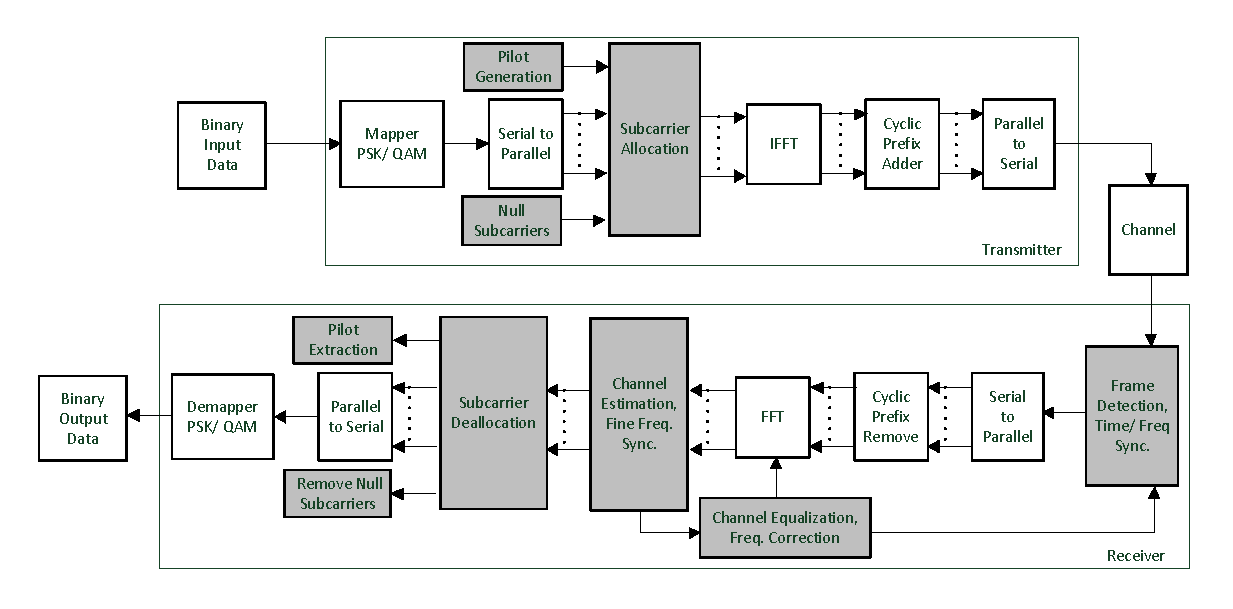
\includegraphics[width=\textwidth]{content/fig/practical_bb_ofdm.pdf}
\caption{Architecture of an OFDM system}
\label{fig:arch_ofdm_sys}
\end{figure}

Considering the radio frequency parts, Figure \ref{fig:tx_rx_ofdm_phy} is concluded \cite{802_11}.\\
 
\begin{figure}[h!]
\centering
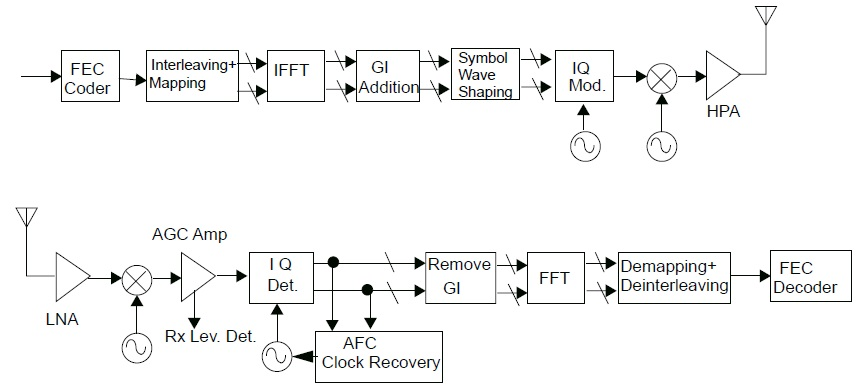
\includegraphics[width=12cm]{content/fig/tx_rx_ofdm_phy.jpg}
\caption{Transmitter and receiver block diagram of OFDM PHY}
\label{fig:tx_rx_ofdm_phy}
\end{figure}



At the receiver side, the frame synchronization and detection for both timing and frequency is performed in the first stage. Channel estimation is performed after the FFT block outputs the preambles in the frequency domain. The result is fed back to the FFT block for the equalization, which eliminates the effects of fading channel, while the fine synchronization for both timing and frequency is also added to further improve the system performance.\\
At least these basic parameters should be specified for a system design:

\begin{enumerate}
  \item Delay spread expected for the channel ($300 ns$)
  \item Guard duration ($800 ns$) which describes symbol duration ($4.0 \mu s$)
  \item Available bandwidth
  \item Data rate
\end{enumerate}

For indoor environment a delay spread less than 300 ns expected. We consider the guard duration 800 ns, which effectively protects the signal from ISI in the indoor environment and some of the outdoor wireless communication environments. Five times the guard duration for limiting the power and bandwidth loss is regarded for the symbol duration, and is set to 4.0 $\mu$s in our case. Hence, the OFDM symbol rate is 0.25 mega symbol per second (Mbaud).\\
Keep in mind, the useful OFDM symbol duration without the guard interval is 3.2 $\mu$s. So, the subcarrier spacing, which is the reciprocal of the useful symbol duration, can be determined as 312.5 kHz. Assuming that there is a bandwidth of 20 MHz available, the number of subcarriers is calculated to be 64. This is exactly the same as the specification defined in IEEE 802.11a standard.\\
As mentioned, some tones are reseved for pilot subcarries (channel estimation), null subcarriers (realizing oversampling to avoid aliasing) and windowing (reduce the out-of-band spectral energy).\\
In our design we chose 48 data tones and 4 pilot subcarriers. So, 52 subcarries are occupied. Applying a raised-cosine window with roll-off factor $\beta$= 0.02 the total occupied bandwidth is\\

\begin{equation} \label{occupied_bw}
(1+ 0.02)\times(52 \times 312.5kHz) \approx 16.6MHz
\end{equation}

To accomplish Oversampling, some zeros before and after the data vector are appended in the frequency domain as shown below.\\

\begin{equation} \label{over_sample}
\overbrace{0, 0, ... , 0,}^{1/2\;appended\;zeros}
\underbrace{d_{-\frac{N_d}{2}}, d_{-\frac{N_d}{2}+1}, ... , d_{-1},}_{Negative\;subcarriers}
\underbrace{d_{1}, d_{2}, ... , d_{\frac{N_d}{2}},}_{Positive\;subcarriers}
\overbrace{0, 0, ... , 0}^{1/2\;appended\;zeros}
\end{equation}

In the IEEE 802.11a transmitter, a 64 point IFFT multiplexes the orthogonal sub-carriers and the sub-carriers are renumbered as in Figure \ref{fig:freq_alloc} before performing the Fourier transformation. Only 48 of them are used for data transmission and they are modulated by using BPSK, QPSK, 16-QAM or 64-QAM according to the Rate parameter. The sub-carriers $P_{-21}$, $P_{-7}$, $P_{7}$ and $P_{21}$ are dedicated to comb-type pilot signals which are used to track the phase variations due to the time varying channel or a frequency o set error. The pilot sub-carriers are modulated by using BPSK and to prevent the generation of spectral lines, they transmit a pseudo random binary sequence generated by the same polynomial used in the scrambler.\\

\begin{figure}[h!]
\centering
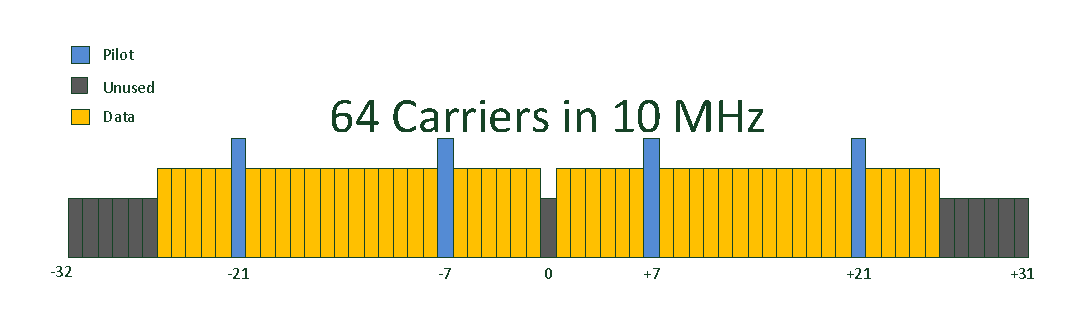
\includegraphics[width=\textwidth]{content/fig/freq_alloc.pdf}
\caption{The frequency allocation of IEEE 802.11a sub-carriers}
\label{fig:freq_alloc}
\end{figure}

The nonzero data values are mapped onto the subcarriers around 0 Hz, and the zeros are mapped onto frequencies around sampling rate.
Basically, in the BPSK modulation is applied on each subcarrier, each symbol for an individual subcarrier has one bits. The bit rate achieves without channel coding:\\

\begin{equation} \label{bitrate_achiv}
\frac{1}{4.0\mu s} \times 48 \times 1= 12Mbps
\end{equation}

The same calculation can be perform for QPSK to reach 24Mbps. But, channel coding will reduce this values. Variation of coding rates and modulation methods, In the 802.11a standard, the data rate ranges from 6 Mbps to 54 Mbps.\\

\begin{table}
\centering
\vspace{0.5cm}
\begin{tabular}{c|c|c}
Parameter&Description&Value\\ \hline
$B_{w}$&Available channel bandwidth&$20MHz$\\
$\sigma_{\tau}$&Delay spread of the channel& $<300 ns$\\
$T_{g}$&Guard interval duration (Cyclic Prefix)&$0.8\mu s$\\
$T_{sym}$&OFDM symbol period&$4.0\mu$\\
$T$&Effective symbol duration (FFT period)&$3.2\mu s (=T_{g}- T_{sym})$\\
$\Delta f$&Subcarrier spacing&$312.5kHz (=1/T)$\\
$N_{g}$&Number of guard samples&$16$\\
$N$&FFT size&$64= B/\Delta f s$\\
$N_{d}$&Number of data subcarriers&$48$\\
$N_{p}$&Number of pilot sucarriers&$4$\\
$N_{u}$&Number of used subcarriers&$52$\\
$B_{u}$&Signal occupied bandwidth&$16.6MHz$\\
&Modulation type&$BPSK, QPSK$\\
$R_{b}$&Data rate without coding&$12Mbps, 24Mbps$\\
\end{tabular}
\caption{System parameters defined for the proposed OFDM system}
\label{table:sys_param}
\end{table}

Table \ref{table:code_vs_rate} shows the length parameter indicates the number of information bytes with different code rates:

\begin{table}
\centering
\vspace{0.5cm}
\begin{tabular}{c|c|c|c|c}
Data rate&Modulation&Code Rate&Coded bits per symbol&Data bits per symbol\\ \hline
6 Mbps&BPSK&1/2&48&24\\
9 Mbps&BPSK&3/4&48&36\\
12 Mbps&QPSK&1/2&96&48\\
18 Mbps&QPSK&3/4&96&72\\
24 Mbps&16QAM&1/2&192&96\\
36 Mbps&16QAM&3/4&192&144\\
\end{tabular}
\caption{Rate dependant parameters in IEEE 802.11a Standard \cite{802_11}}
\label{table:code_vs_rate}
\end{table}

The theoretical equation of the Bit-Error Rate for a QPSK channel is:\\

\begin{equation} \label{theo_ber}
P_{b}(e)= \dfrac{1}{2}erfc(\sqrt{\dfrac{E_{b}}{N_{0}}})
\end{equation}

It is discussed that the BER can be computed by considering the non-ideality which the two parameters \textit{guard time} and \textit{pilots} will inject into the result. The formulation would be:\\

\begin{equation} \label{theo_ber_guard_pilot}
P_{b}(e)= \dfrac{1}{2}erfc(\sqrt{\dfrac{E_{b}}{N_{0}}\dfrac{T}{T+T_{g}}\dfrac{N_{u}}{N_{u}+N_{p}}})
\end{equation}

Replacing the standard value from Table \ref{table:sys_param} in the equation we have:\\

\begin{equation} \label{theo_ber_ieee}
P_{b}(e)= \dfrac{1}{2}erfc(\sqrt{\dfrac{E_{b}}{N_{0}}0.65})
\end{equation}

\subsection{IEEE 802.11a Standard in Time and Frequency}
\label{section:ieee_standard}
A packet of OFDM will be described here. In an OFDM frame, a preamble which carries no data is transmitted first, followed by the signal field which give some information about data and transmitted data. An OFDM frame has the general form as below:
\begin{equation} \label{sym_ofdm}
s_{OFDM}(t)= s_{preamble}(t)+ s_{signal}(t- T_{preamble})+ s_{data}(t- T_{preamble}- T_{signal})
\end{equation}

where\\
\begin{equation} \label{preamble_ofdm}
s_{preamble}(t)= s_{short}(t)+ s_{long}(t- T_{short})
\end{equation}

As shown in Figure \ref{fig:preamble_ieee}, the preamble starts with 10 short training symbols (STSs) from $T_{1}$ to $T_{10}$, followed by a guard interval ($GI_{2}$) and two long training symbols (LTSs) $L_{1}$ and $L_{2}$. Both the short and long training sequences have an $8 \mu s$ duration and the entire preamble lasts for $16 \mu s$. Then, a $3.2 \mu s$ signal symbol, as well as 800 ns guard interval is transmitted. This field bears some information necessary for the data symbols, such as the coding rate and length. Finally the various data symbols that carry user information are transmitted. Each data symbol has a duration of $4.0 \mu s$, within which there is a 800 ns CP, as already described.\\
The application of STS and LTS for training are different. STS used for AGC, frame detection, coarse timing and frequency synchronization. Each symbol in this sequence has a duration of 800 ns and contains 16 samples, and is identical to one another.
 It will be shown in a professional system, auto-correlation will apply to this portion to perform such the operations. After the short training sequence is transmitted, a $1.6 \mu s$ guard interval that contains 32 samples is introduced. The LTS is cyclically extended within this interval. Then two identical LTSs with the same duration of $4.0 \mu s$ are followed. The LTS is used for fine frequency offset and channel estimation. It will be described that a cross-correlation with a stored array is done for extraction of the offset.\\
The data being transmitted should pass several stages and be prepared by PLCP (Physical Layer Convergence Procedure) before transmission. The preamble and the PLCP header are transmitted at 1Mbps regardless of the current data transmission speed. After the preamble the payload prepared by the MAC layer is sent to the receiver at the rate specified in the services field.\\
The picture below shows the OFDM packet data layout. It starts with training sequence (PLCP preamble), followed by the SIGNAL field and data. The data is followed by 6 tail bits and padding (not shown on the picture). Both the training sequence and the 24 bit SIGNAL field are transmitted at $6 Mbps$ rate. The SIGNAL field tells the receiver at what rate the following data will be transmitted and indirectly defines the subcarriers' modulation technique employed. The BPSK, QPSK, 16-QAM and 64-QAM are the available choices. The SIGNAL field also delivers the length (12 bit) of the following data and includes a zero bit sequence for the data scrambler synchronization. The total training sequence and SIGNAL field transmission times add up to about $20 \mu s$, which is an overhead equivalent to approximately 140 bytes transmission at the maximum transmission rate of 54Mbps defined by the standard.\\

\begin{figure}[h!]
\centering
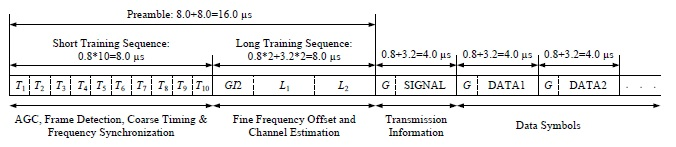
\includegraphics[width=\textwidth]{content/fig/ofdm_frame.JPG}
\caption{Preamble of IEEE 802.11 \cite{802_11}}
\label{fig:preamble_ieee}
\end{figure}


As we already analyzed, 52 subcarriers are used for an OFDM data symbol and pilot. Oversampling is achieved by adding 12 null subcarriers in order to eliminate aliasing which might occur during digital to analog conversion. Because FFT shift is performed, the null subcarriers with a value of zero are located in the middle of the input vector for the IFFT block. Note that dc carrier is not used to transmit data. The short and long training sequences can also be applied to this mapping rule, since they both have a length of 52 samples with frequency index from -26 to +26.\\


\subsection{Origin of CFO}
A simple model of a radio transmitter and receiver can depict the basis of the CFO source. \cite{tse} \cite{salehi}

\begin{figure}[h!]
\centering
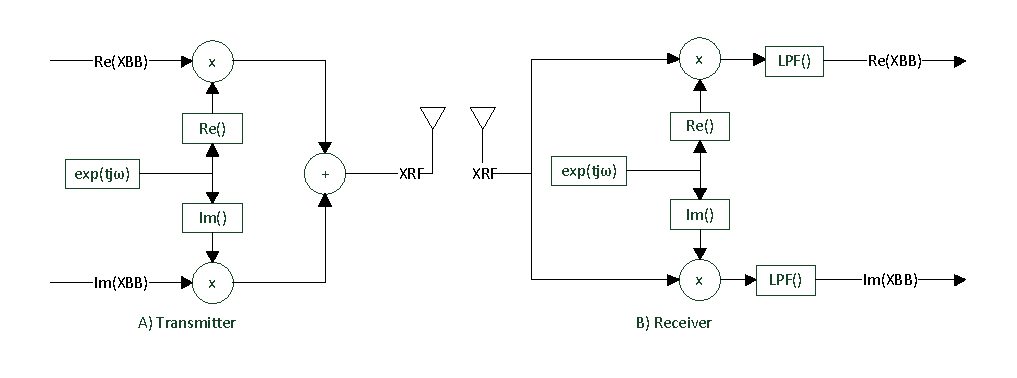
\includegraphics[width=\textwidth]{content/fig/drct_rf_mdl.pdf}
\caption{General models of a direct conversion RF}
\label{fig:cfo_radio_model}
\end{figure}

In Figure \ref{fig:cfo_radio_model}, $\omega$ is The carrier frequency and $X_{BB}$ is the complex baseband signal, $X_{RF}$ is
a real-valued RF signal. These models simplified many other operations in a real RF transceivers although none of these affect the up/down-conversion processes as they relate to CFO.\\
These equations about transmit and receive processes can be written in equation (\ref{eq_tx_rx_process}):

\begin{equation}\label{eq_tx_rx_process}
\begin{split}
X_{RF} & = TX(X_{BB})\\
& = Re(X_{BB})\cos(\omega t) - Im(X_{BB})\sin(\omega t)\\
& = \frac{1}{2} (X_{BB} e^{jt\omega} + X^{*}_{BB} e^{-jt\omega})\\
\\
X_{BB} & = RX(X_{RF}, \omega)\\
& = LPF(X_{RF} e^{j\omega t})
\end{split}
\end{equation}


Assume a signal $S_{BB}$ transmitted with carrier frequency $\omega_{S}$ which is received with carrier frequency $\omega_{D}$. we can express the received baseband signal $D_{BB}$ in terms of the transmitted baseband signal $S_{BB}$ and the carrier frequencies. Then:\\

\begin{equation} \label{DBB_SBB}
\begin{split}
D_{BB} & = LPF(\frac{(S_{BB} e^{jt\omega_{S}} + S^{*}_{BB} e^{-jt\omega_{S}})e^{jt\omega_{D}}}{2})\\
&= S_{BB}(e^{jt(\omega_{S}- \omega_{D})})
\end{split}
\end{equation}

The received baseband signal is equal to the original baseband signal modulated by a complex sinusoid. In the frequency domain, this gives a received spectrum equal to the transmitted one, only shifted away from DC by the difference in the carrier frequencies of the transmitter and receiver (i.e. $\omega_{S}- \omega_{D}$). This shift of the received
signal is the baseband manifestation of carrier frequency offset.

\subsection{Impact of CFO}
\label{Impact_of_CFO}
There are two destructive impacts on an OFDM system. Firstly, the phase offset across subcarriers in an symbol which can be  estimated and corrected in frequency domain to prevent errors in a constant rotated constellation. Some subcarriers are allocated as pilot tones which receiver can estimate phase errors.\\
The second effect of CFO is the degradation of orthogonality between subcarriers in receiver's FFT which causes inter-carrier interference (ICI). ICI acts an effective SNR reduction as a result of CFO increasing.\\
The impact is displayed in Figure \ref{fig:cfo_impact_on_ici} which is shown simulated OFDM system uses 10 MHz bandwidth and 64 subcarriers, 48 of on a random 16-QAM data symbols. CFO and AWGN are applied between the transmitter and receiver. The receiver model uses perfect knowledge of the CFO to correct the phase offset in each OFDM symbol, but does not implement any correction for ICI. \cite{murphy_thesis}\\

\begin{figure}[h!]
\centering
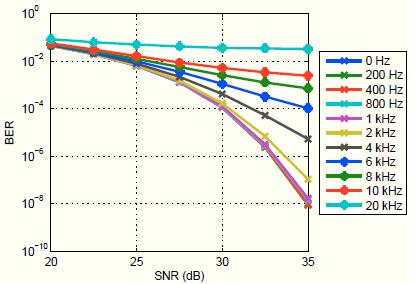
\includegraphics[width=10cm]{content/fig/cfo_on_ici.JPG}
\caption{OFDM performance loss due to CFO-induced ICI.\cite{murphy_thesis}}
\label{fig:cfo_impact_on_ici}
\end{figure}

The results shows that for large CFOs errors caused by ICI dominate performance, even at high SNR. It is also
clear that for small CFOs performance is dominated by SNR. Specifically, for frequency offsets smaller than 1 kHz, the
performance degradation due to ICI is negligible.\\

\begin{figure}[h!]
\centering
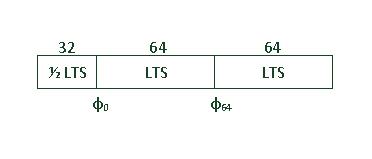
\includegraphics{content/fig/lts_time_domain.pdf}
\caption{LTS in Time Domain.}
\label{fig:lts_time_domain}
\end{figure}

Let's focus on LTS part in a OFDM symbol, Figure \ref{fig:lts_time_domain}, for a while. In time domain, we have 160 samples in this section which creates to complete LTS symbols and a half and each LTS symbol has 64 samples.\\

We can say:
\begin{equation} \label{cfo_cal}
\begin{split}
CFO \approx (\phi_{64}- \phi_{0})\\
CFO_{EST} = \frac{f_{s}}{2\pi . 64^{2}} \sum\limits_{n=64}^{127} \phi_{n}- \phi_{(n-64)}\\
\end{split}
\end{equation}


\begin{figure}[h!]
\centering
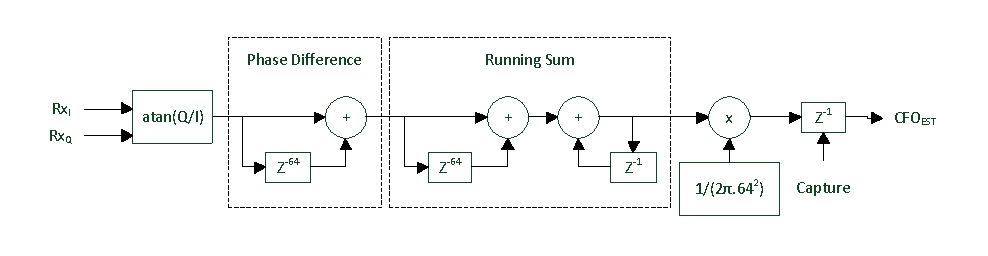
\includegraphics{content/fig/time_dom_cfo_est.pdf}
\caption{Time Domain CFO Estimation.}
\label{fig:cfo_est}
\end{figure}

Which $CFO_{EST}$ is the estimated CFO. To have such the structure in the Simulink we can arrange as Figure \ref{fig:cfo_est}.

\subsection{Synchronization}
\label{section:sync}

The synchronization tasks is challenging in an OFDM-based communication system. Prior to performing channel estimation equalization and demodulation, OFDM symbol timing must be detected. The receiver has no information when a packet starts, and so the first synchronization task is packet detection. Once a packet has been detected the remaining synchronization functions include coarse and fine timing recovery and carrier recovery.\\
Figure \ref{fig:preamble_ieee} shows the structure of the IEEE 802.1la standard preamble. The 10 short preambles ($t_{1}$-$t_{10}$) are identical 16- sample duration sequences. The cyclic prefix ($GI2$) is a 32- sample sequence and the long preambles ($T_{1}$ and $T_{2}$) are identical 64-sample sequences. As indicated in the figure, the various fields are used for packet detection, automatic gain control (AGC), diversity selection, coarse and fine frequency offset estimation, fine symbol timing estimation and channel estimation.\\

The packet detector is based on the Schimdl and Cox delay and correlate algorithm employed for acquiring symbol timing commonly. \cite{sch_cox} The algorithm, as illustrated in Figure \ref{fig:schimdl_cox}, is basically a sliding window correlator combined with an energy detector used to normalize the decision statistic and hence guard against fluctuations of the input signal power level. \cite{dick}\\

The sliding window P computes a auto-correlation between the input signal and a D-sample delayed version on short preamble interval. We chose D=16. The second sliding window R is used to compute the received signal energy in the cross-correlation interval.

\begin{equation} \label{P_n}
P(n) = \sum\limits_{m=0}^{L-1} r_{n+m} r^{*}_{n+m+D}
\end{equation}

\begin{equation} \label{R_n}
 R(n) = \sum\limits_{m=0}^{L-1} r_{n+m+D} r^{*}_{n+m+D}
\end{equation}

The cross-correlation P(n) and auto-correlation R(n) are calculated according to Equation \ref{P_n} and Equation \ref{R_n} respectively. The decision statistic is computed as\\

\begin{equation} \label{M_n}
M(n)= \dfrac{|P(n)|^{2}}{R(n)^{2}}
\end{equation}

\begin{figure}[h!]
\centering
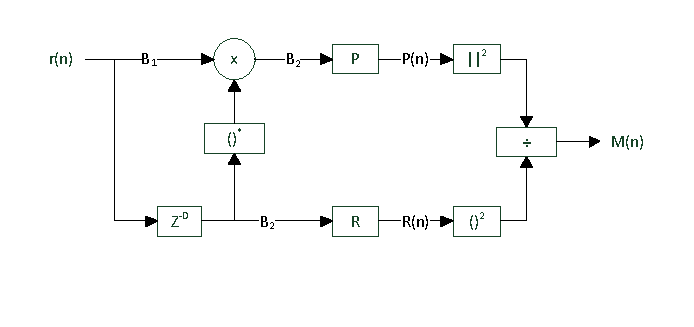
\includegraphics[width=\textwidth]{content/fig/schl_cox_mdl.pdf}
\caption{Schimdl and Cox Delay and Correlate Algorithm.}
\label{fig:schimdl_cox}
\end{figure}

\subsection{Channel Estimation and Distortion Reject}
\label{section:channel_est}

Imagine the estimated channel is $\hat{H}$ and the input information is $A$. So, we can expect to compensate the signal as below:\\

\begin{equation} \label{channel_Comp}
\begin{split}
A_{compensate} & = \dfrac{A}{\hat{H}}\\
&= \dfrac{A.{\hat{H}}^*}{|\hat{H}|}
\end{split}
\end{equation}

If the estimasion is done correctly and the channel is perfect without any distortion, we expect $\hat{H}$ to be a flat shape in whole frequencies. Such the estimation is done by LTS to have the same input on all the tones at the transmitter and calculate the channel in the receiver by studying LTS.\\